\documentclass[journal]{IEEEtran}
\usepackage[a5paper, margin=10mm]{geometry}
%\usepackage{lmodern} % Ensure lmodern is loaded for pdflatex
\usepackage{tfrupee} % Include tfrupee package


\setlength{\headheight}{1cm} % Set the height of the header box
\setlength{\headsep}{0mm}     % Set the distance between the header box and the top of the text


%\usepackage[a5paper, top=10mm, bottom=10mm, left=10mm, right=10mm]{geometry}

%
\setlength{\intextsep}{10pt} % Space between text and floats

\makeindex


\usepackage{cite}
\usepackage{amsmath,amssymb,amsfonts,amsthm}
\usepackage{algorithmic}
\usepackage{graphicx}
\usepackage{textcomp}
\usepackage{xcolor}
\usepackage{txfonts}
\usepackage{listings}
\usepackage{enumitem}
\usepackage{mathtools}
\usepackage{gensymb}
\usepackage{comment}
\usepackage[breaklinks=true]{hyperref}
\usepackage{tkz-euclide} 
\usepackage{listings}
\usepackage{multicol}
\usepackage{xparse}
\usepackage{gvv}
%\def\inputGnumericTable{}                                 
\usepackage[latin1]{inputenc}                                
\usepackage{color}                                            
\usepackage{array}                                            
\usepackage{longtable}                                       
\usepackage{calc}                                             
\usepackage{multirow}                                         
\usepackage{hhline}                                           
\usepackage{ifthen}                                               
\usepackage{lscape}
\usepackage{tabularx}
\usepackage{array}
\usepackage{float}
\usepackage{ar}
\usepackage[version=4]{mhchem}


\newtheorem{theorem}{Theorem}[section]
\newtheorem{problem}{Problem}
\newtheorem{proposition}{Proposition}[section]
\newtheorem{lemma}{Lemma}[section]
\newtheorem{corollary}[theorem]{Corollary}
\newtheorem{example}{Example}[section]
\newtheorem{definition}[problem]{Definition}
\newcommand{\BEQA}{\begin{eqnarray}}
\newcommand{\EEQA}{\end{eqnarray}}

\theoremstyle{remark}


\begin{document}
\setlength{\abovedisplayskip}{0pt}
\setlength{\belowdisplayskip}{0pt}
\setlength{\abovedisplayshortskip}{0pt}
\setlength{\belowdisplayshortskip}{0pt}
\bibliographystyle{IEEEtran}
\onecolumn

\title{2.2.24}
\author{Jnanesh Sathisha Karmar- EE25BTECH11029}
\maketitle


\renewcommand{\thefigure}{\theenumi}
\renewcommand{\thetable}{\theenumi}
\textbf{Question}Show that the points $\brak{1, 7}$, $\brak{4, 2}$, $\brak{-1, -1}$ and $\brak{-4, 4}$ are the vertices of a square.

\textbf{Solution}
Given details:
\begin{align}
    \vec{A}=\myvec{1\\7}  \vec{B}=\myvec{4\\2} \vec{C}=\myvec{-1\\-1} \vec{D}=\myvec{-4\\4}
\end{align}

Find the sides
\begin{align}
\vec{B}-\vec{A}=\myvec{3\\-5} \  \vec{C}-\vec{B}=\myvec{-5\\-3} \\
\vec{D}-\vec{C}=\myvec{-3\\5} \ 
\vec{A}-\vec{D}=\myvec{5\\3}
\end{align}
First let's check wheter the given opposite sides of the polygon are parallel to each other \\
For the sides to be parallel 
\begin{align}
    \vec{B-A}=\vec{D-C}\\
    \vec{C-B}=\vec{A-D}\\
\end{align}
Since:
\begin{align}
    \vec{B-A}=\vec{C-D}=\myvec{3\\-5}\\
    \vec{C-B}=\vec{D-A}=\myvec{-5\\-3}
\end{align}
Therefore the opposite sides are parallel to each other and Thus the given polygon can be classified as a \textbf{Parallelogram}.\\
Now put these sides as columns of a $2\times4$ matrix V:
\begin{align}
    \vec{V}=\myvec{B-A&C-B&D-C&A-B}\\
    =\myvec{3 & -5 & -3 & 5\\-5 & -3 & 5 & 3}
\end{align}
Compute the $4\times4$Gram matrix $\vec{G}=\vec{V^TV}$.Its entries are all possible inner products\\


Adjacent inner products of the Gram matrix would be\brak{\text{off-diagonals for consecutive sides}}:
\begin{align}
\brak{\vec{B-A}^T}\brak{\vec{C-B}} = 3\brak{-5} + \brak{-5}\brak{-3} = -15 + 15 = 0\\
\brak{\vec{C-B}^T} \brak{\vec{D-C}} = \brak{-5}\brak{-3} + \brak{-3}(5) = 15 - 15 = 0,\\
\brak{\vec{D-C}^T} \brak{\vec{A-D}} = \brak{-3}(5) + 5(3) = -15 + 15 = 0,\\
\brak{\vec{A-D}^T} \brak{\vec{B-A}} = 5(3) + 3\brak{-5} = 15 - 15 = 0.
\end{align}
Since all are zero ,it means all the sides are perpendicular to each other . Therefore the given parallelogram can be classified as a \textbf{Rectangle}.

In the matrix G self inner-products would be 
\brak{\text{diagonal of G}}:

\begin{align}
    {\brak{\vec{A-B}}^T\brak{\vec{A-B}}}={3^2+\brak{-5}^2}={34}\\
    {\brak{\vec{B-C}}^T\brak{\vec{B-C}}}={\brak{-5}^2+\brak{-3}^2}={34}\\
    {\brak{\vec{C-D}}^T\brak{\vec{C-D}}}=\brak{-3}^2+5^2={34}\\
    \brak{\vec{D-A}}^T\brak{\vec{D-A}}=5^2+3^2=34
\end{align}
since all are equal to 34 , it means all the side lengths are equal , therefore the given rectangle can be classified as a \textbf{Square}. 



\begin{figure}[H]
    \centering
    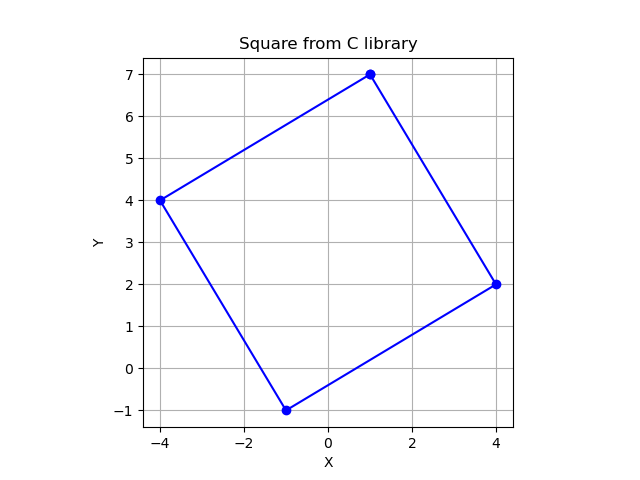
\includegraphics[width=1\columnwidth]{figs/square.png}
    \caption{Sqaure}
    \label{fig:placeholder_1}
\end{figure}
\end{document}